\documentclass[12pt,a4paper]{article}

\usepackage{graphicx}% Include figure files
\usepackage{dcolumn}% Align table columns on decimal point
\usepackage{bm}% bold math
%\usepackage{hyperref}% add hypertext capabilities
%\usepackage[mathlines]{lineno}% Enable numbering of text and display math
%\linenumbers\relax % Commence numbering lines

%\usepackage[showframe,%Uncomment any one of the following lines to test 
%%scale=0.7, marginratio={1:1, 2:3}, ignoreall,% default settings
%%text={7in,10in},centering,
%%margin=1.5in,
%%total={6.5in,8.75in}, top=1.2in, left=0.9in, includefoot,
%%height=10in,a5paper,hmargin={3cm,0.8in},
%]{geometry}

\usepackage{multicol}%Para hacer varias columnas
\usepackage{multicol,caption}
\usepackage{multirow}
\usepackage{cancel}
\usepackage{hyperref}
\hypersetup{
    colorlinks=true,
    linkcolor=blue,
    filecolor=magenta,      
    urlcolor=cyan,
}

\setlength{\topmargin}{-1.0in}
\setlength{\oddsidemargin}{-0.3pc}
\setlength{\evensidemargin}{-0.3pc}
\setlength{\textwidth}{6.75in}
\setlength{\textheight}{9.5in}
\setlength{\parskip}{0.5pc}

\usepackage[utf8]{inputenc}
\usepackage{expl3,xparse,xcoffins,titling,kantlipsum}
\usepackage{graphicx}
\usepackage{xcolor} 
\usepackage{siunitx}
\usepackage{nopageno}
\usepackage{lettrine}
\usepackage{caption}
\renewcommand{\figurename}{Figura}
\usepackage{float}
\renewcommand\refname{Bibliograf\'ia}
\usepackage{amssymb}
\usepackage{amsmath}
\usepackage[rightcaption]{sidecap}
\usepackage[spanish]{babel}

\providecommand{\abs}[1]{\lvert#1\rvert}
\providecommand{\norm}[1]{\lVert#1\rVert}
\newcommand{\dbar}{\mathchar'26\mkern-12mu d}

% CABECERA Y PIE DE PÁGINA %%%%%
\usepackage{fancyhdr}
\pagestyle{fancy}
\fancyhf{}

\begin{document}

Macías Márquez Misael Iván

\begin{enumerate}



%%%1%%%



    \item La primer ley de la termodinámica nos ofrece la siguiente relación:
    
    \begin{equation*}
        dU = \dbar Q + dW
    \end{equation*}
    
    \begin{enumerate}
        \item  Explique breve y concisamente la interpretación física de la expresión anterior
        
        \textbf{Sol:}
        
        La expresión anterior describe la relación entre la energía mecánica (trabajo) y no mecánica (calor) con la energía interna de un sistema que podría verse como su energía total 
        
        \item ¿Se puede considerar la energía como la suma de una componente calor y una componente de trabajo?
        
        No del todo porque podrian existir otras formas de energía presentes, como la debida al potencial químico, etc
    \end{enumerate}
    
    
    
%%%2%%%
    
    
    
    \item A partir de la primera ley demuestre la relación:
    
    \begin{equation*}
        \dbar Q = C_P d\theta - \frac{\kappa_\theta}{\beta}(C_P - C_V) dP
    \end{equation*}
    
    \textbf{Sol:}
    
    por la primera ley tenemos que 
    
    \begin{equation}
        \dbar Q =  p dV + dU
    \end{equation}
    
    ahora como
    
    \begin{equation*}
        dV = \left(\frac{\partial V}{\partial \theta}\right)_p d\theta + \left(\frac{\partial V}{\partial p}\right)_\theta dp
    \end{equation*}
    
    \begin{equation*}
        dU = \left(\frac{\partial U}{\partial \theta}\right)_p d\theta + \left(\frac{\partial V}{\partial p}\right)_\theta dp
    \end{equation*}
    
    si sustituimos en (1)
    
    \begin{equation*}
        \dbar Q = p \left[\left(\frac{\partial V}{\partial \theta}\right)_p d\theta + \left(\frac{\partial V}{\partial p}\right)_\theta dp \right] + \left(\frac{\partial U}{\partial \theta}\right)_p d\theta + \left(\frac{\partial V}{\partial p}\right)_\theta dp
    \end{equation*}
    
    \begin{equation}
        \dbar Q = \left[p\left(\frac{\partial V}{\partial \theta}\right)_p + \left(\frac{\partial U}{\partial \theta}\right)_p \right] d\theta + \left[p\left(\frac{\partial V}{\partial p}\right)_\theta + \left(\frac{\partial V}{\partial p}\right)_\theta\right] dp
    \end{equation}
    
    ahora si derivamos (2) respecto a $\theta$ con $p$ constante y sustituimos en (2)
    
    \begin{equation*}
        \left(\frac{\dbar Q}{d \theta}\right)_p = p\left(\frac{\partial V}{\partial \theta}\right)_p + \left(\frac{\partial U}{\partial \theta}\right)_p = C_p
    \end{equation*}
    
    \begin{equation}
        \dbar Q = C_p d\theta + \left[p\left(\frac{\partial V}{\partial p}\right)_\theta + \left(\frac{\partial V}{\partial p}\right)_\theta\right] dp
    \end{equation}
    
    si derivamos (3) respecto a $\theta$ con $V$ constante y usamos $\left(\frac{dp}{d\theta}\right)_V = \frac{\beta}{\kappa_\theta}$
    
    \begin{equation*}
        \left(\frac{\dbar Q}{d \theta}\right)_V = C_p + \left[p\left(\frac{\partial V}{\partial p}\right)_\theta + \left(\frac{\partial V}{\partial p}\right)_\theta\right] \left(\frac{dp}{d\theta}\right)_V = C_V 
    \end{equation*}
    
    \begin{equation*}
        \left[p\left(\frac{\partial V}{\partial p}\right)_\theta + \left(\frac{\partial V}{\partial p}\right)_\theta\right] = -(C_p - C_v) \frac{1}{\left(\frac{dp}{d\theta}\right)_V}= -(C_p - C_v) \frac{\kappa_\theta}{\beta}
    \end{equation*}
    
    \begin{equation*}
        \therefore  \dbar Q = C_p d\theta  -(C_p - C_v) \frac{\kappa_\theta}{\beta} dp
    \end{equation*}
    
    
    
%%%3%%%
    
    
    
    \item En un metal a bajas temperaturas la capacidad calorífica a volumen constante varía con la temperatura de acuerdo con la siguiente ecuación:
    
    \begin{equation*}
        \frac{C_V}{n} = \left(\frac{124.8}{\Theta}\right)^3 \frac{mJ}{mol \cdot K} T^3 + \gamma T
    \end{equation*}
    
    donde $\Theta$ se conoce como la temperatura de Debye y $\gamma$ es una constante con las unidades adecuadas. Para el cobre se tiene
    
    \begin{equation*}
        \Theta = 343 K \hspace{2cm} \gamma = 0.688 \frac{mJ}{mol \cdot K^2}
    \end{equation*}
    
    ¿Cuánto calor por mol es transferido en un proceso en el que la temperatura cambia de $1.7 K$ a $2.3 K$?
    
    Recuerde que las unidades de $\frac{C_V}{n}$ son $\frac{mJ}{mol \cdot K}$.
    
    Dado que $C_V=\left(\frac{\partial Q}{\partial T}\right)_V$, entonces el calor por mol en un proceso de $1.7 K$ a $2.3 K$ es 
    
    \begin{equation*}
        \int_{1.7K}^{2.3K} dT \frac{C_V}{n}= \left(\frac{124.8}{\Theta}\right)^3 \frac{mJ}{mol \cdot K} \int_{1.7K}^{2.3K} dT    T^3 + \gamma \int_{1.7K}^{2.3K} dT  T
    \end{equation*}
    
    \begin{equation*}
        = \left(\frac{124.8}{\Theta}\right)^3 \frac{mJ}{mol \cdot K} \left(\frac{(2.3K)^4}{4} - \frac{(1.7K)^4}{4}\right) + \gamma \left(\frac{(2.3K)^{2}}{2} - \frac{(1.7K)^{2}}{2} \right)
    \end{equation*}
    
    \begin{equation*}
        =\frac{1227}{250} \left(\frac{124.8}{\Theta}\right)^3 \frac{mJ K^3}{mol \cdot}  +  \frac{6\gamma}{5} K^2
    \end{equation*}
    
    \begin{equation*}
        \approx (0.24 + 0.83) \frac{mJ}{mol} = 1.07   \frac{mJ}{mol}
    \end{equation*}
    
    
    
%%%4%%%
    
    
    
    \item Sea un gas encerrado en un cilindro con un pistón movible. Se observa que, si las paredes son adiabáticas, un incremento cuasi-estático en el volumen resulta en un decremento en la presión de acuerdo con la ecuación
    
    \begin{equation}
        P^3 V^5 = cte
    \end{equation}
    
    Considere los siguientes estados del sistema:
    
    \begin{enumerate}
        \item A: un estado con volumen $10^{-3} m^3$ y presión $10^5$ Pa.
        
        \item B: un estado con volumen $\num{8 e -3}m^3$ y presión $10^5/32$ Pa.
        
        \item C: un estado con volumen igual al de A y presión igual a la de B.
        
        \item D: un estado con volumen igual al de B y presión igual a la de A
        
        
        \begin{enumerate}
            \item Dibuje el diagrama, en el espacio fase, de los procesos ADB, ACB, AB y l proceso dado por la ec. (4).
            
            \begin{figure}[h!]
                \centering
                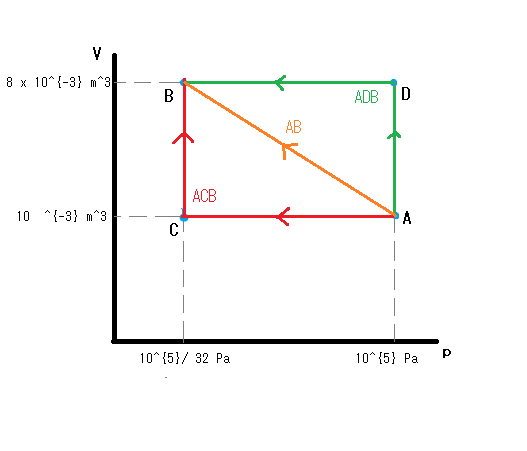
\includegraphics[scale = 0.8]{ACBADB.png}
            \end{figure}
            
            Si despejamos $V$ de la ec. (4) obtenemos una hipérbola 
            
            \begin{figure}[h!]
                \centering
                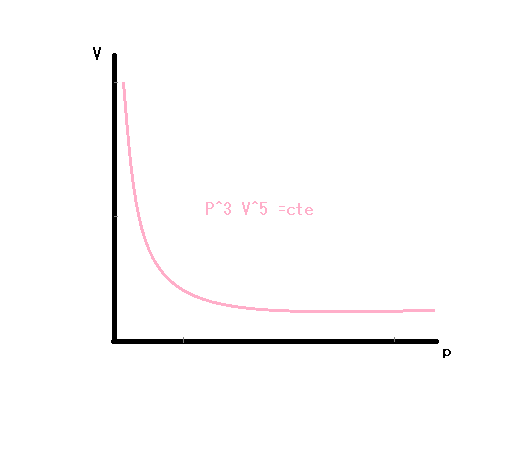
\includegraphics[scale = 0.8]{pv.png}
            \end{figure}
            
            \newpage
            
            \item Encuentre el trabajo cuasi-estático realizado y el calor neto transferido en cada uno de los procesos: ADB, ACB y AB (siguiendo la línea recta que conecta estos dos puntos en el espacio fase).
            
            El trabajo cuasi-estático está determinado por $ W = \int pdV$), entonces
            
            \begin{equation*}
                ADB \hspace{0.2cm} \rightarrow  \hspace{0.2cm} W_{ADB} =  W_{AD} + \cancel{W_{DB}} = \int_{\num{e-3}m^3}^{\num{8e-3}m^3} P_{cte} dV =  
            \end{equation*}
            
            \begin{equation*}
                =(\num{e5}Pa) (\num{8e-3}m^3 - \num{e-3}m^3) = 700 J
            \end{equation*}
            
            \begin{equation*}
                ACB \hspace{0.2cm} \rightarrow  \hspace{0.2cm} W_{ACB} = \cancel{W_{AC}} + W_{CB} =  \int_{\num{e-3}m^3}^{\num{8e-3}m^3} P'_{cte} dV
            \end{equation*}
            
            \begin{equation*}
                 = (\frac{\num{e5}}{32}Pa) ((\num{8e-3}m^3 - \num{e-3}m^3)) = 21.88 J
            \end{equation*}
            
            \begin{equation*}
                AB \hspace{0.2cm} \rightarrow  \hspace{0.2cm} W_{AB} = 360.94 J
            \end{equation*}
            
             para el calor transferido supongamos que es un gas dicotómico e ideal
             
             \begin{equation*}
                 ADB \hspace{0.2cm} \rightarrow  \hspace{0.2cm} Q_{ADB} = \frac{7}{2} (P_{B}V_{B} - P_{A} V_{A}) = -262.5 J 
             \end{equation*}
             
             \begin{equation*}
                 ACB \hspace{0.2cm} \rightarrow  \hspace{0.2cm} Q_{ACB} = \frac{7}{2} (P_{B}V_{B} - P_{A} V_{A}) = Q_{ADB}
             \end{equation*}
             
             \begin{equation*}
                 AB \hspace{0.2cm} \rightarrow  \hspace{0.2cm} Q_{AB} = \frac{7}{2} (P_{B}V_{B} - P_{A} V_{A}) = Q_{ADB} = Q_{ACB}
             \end{equation*}
             
            
            \item Calcule la energía del estado con $P=\num{5 e 4}Pa$ y $V = \num{8 e -3}m^3$
            
            La verdad no sé a que se refieren pero bueno si uso la ec. (4) las unidades no son de energía, así que creo que no debo usar eso, ahora ya que $PV$ tiene unidades de energía, usaré eso
            
            \begin{equation*}
                P V = (\num{5 e 4}Pa)(\num{8 e -3}m^3) = 400 J = E(?)
            \end{equation*}
        \end{enumerate}
    \end{enumerate}
\end{enumerate}

\end{document}